\documentclass{beamer}
\usepackage[utf8]{inputenc}
\usepackage{float}

\usetheme{Madrid}
\usecolortheme{default}

%Information to be included in the title page:
\title[Geodésica en Espacio de Minkowski] %optional
{Geodésica Alrededor de una Partícula con la Métrica de Schwarzschild}

\author[Garcia, Llanos] % (optional, for multiple authors)
{Manuel Angel Garcia\inst{1} \and Carlos Andres Llanos\inst{2}}

\institute[] % (optional)
{
  Facultad de Física\\
  Universidad Nacional de Colombia \\
  \inst{1} mangarciama@unal.edu.co, \inst{2} cllanos@unal.edu.co
}


\date[2024] % (optional)
{Clase de Objetos Astrofísicos }

\logo{
\includegraphics[height=1cm]{Logo-unal}}

\begin{document}

\frame{\titlepage}

%%%%%%%%%%%%%%%%%%%%%%%%%%%%%%%%%%%%%%%%%%

\begin{frame}
  \tableofcontents
\end{frame}

%%%%%%%%%%%%%%%%%%%%%%%%%%%%%%%%%%%%%%%%%%

\begin{frame}
  \frametitle{Conceptos Preliminares}
  \section{Conceptos Preliminares}
  \textbf{Tensor }
  \begin{figure}
    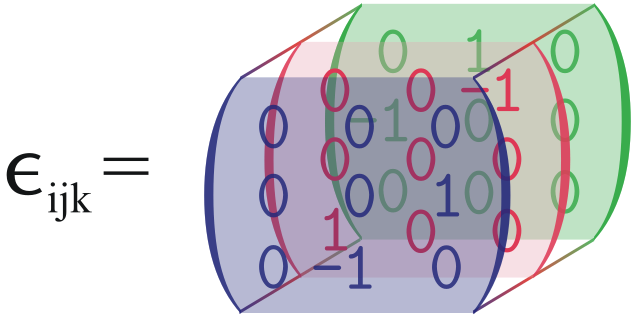
\includegraphics[width=0.45\textwidth]{tensor.png}
  \end{figure}
  
  \textbf{Geodésica }
  \begin{figure}
    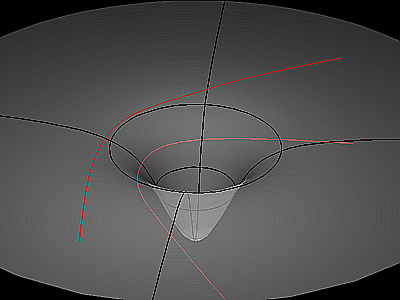
\includegraphics[width=0.45\textwidth]{geodesicas.png}
  \end{figure}
\end{frame}

%%%%%%%%%%%%%%%%%%%%%%%%%%%%%%%%%%%%%%%%%%

\begin{frame}
\frametitle{Métrica de Schwarzschild}
\section{Métrica de Schwarzschild}
\subsection{Métrica de Minkowski}

Partiendo de la métrica de Minkowski en esféricas: 
\begin{gather*}
  ds^2 _{\text{Minkowski }}  = - dt^2 + dr^2 + r^2 d \Omega^2
\end{gather*}

Necesitamos una métrica que mantenga la forma del ángulo solido, así que podemos multiplicarlo por una función radial:
\begin{gather*}
  ds^2 = - e ^ {2 \alpha (r) } dt^2 + e ^ {2 \beta(r) } dr^2 + e ^ {2\gamma(r)}r^2 d \Omega^2 
\end{gather*}

Vamos a imponer que la métrica sea simétrica en sus componentes angulares por lo que la podemos reescribir como:

\begin{gather*}
  ds^2 = - e ^ {2\alpha(r)}dt^2 + e ^ {2 \beta (r) } dr^2 + r^2 d \Omega^2  
\end{gather*}

\end{frame}


%%%%%%%%%%%%%%%%%%%%%%%%%%%%%%%%%%%%%%%%%%


\begin{frame}
\frametitle{Métrica de Schwarzschild}
\subsection{Símbolos de Christoffel y Tensor de Curvatura}

\begin{gather*}
  ds^2 = - e ^ {2\alpha(r)}dt^2 + e ^ {2 \beta (r) } dr^2 + r^2 d \Omega^2  
\end{gather*}
Calculamos los símbolos de Christoffel:
\begin{align*}
  &\Gamma_{t r}^t=\partial _r \alpha \qquad &&\Gamma_{t t}^r=e^{2(\alpha-\beta)} \partial_r \alpha \qquad &&&\Gamma_{r r}^{r}=\partial_r \beta \\
  &\Gamma_{r \theta}^\theta=\frac{1}{r} \qquad &&\Gamma_{\theta \theta}^r=-r e^{-2 \beta} \qquad &&&\Gamma_{r \phi}^\phi=\frac{1}{r} \\
  &\Gamma_{\phi \phi}^r=-r e^{-2 \beta} \sin ^2 \theta \qquad &&\Gamma_{\phi \phi}^\theta=-\sin \theta \cos \theta \qquad &&&\Gamma_{\theta \phi}^\phi=\frac{\cos \theta}{\sin \theta}
\end{align*}
\end{frame}


%%%%%%%%%%%%%%%%%%%%%%%%%%%%%%%%%%%%%%%%%%


\begin{frame}
\frametitle{Métrica de Schwarzschild}

Con los símbolos de Christoffel podemos obtener el tensor de Riemann: 

\begin{align*}
  &R_{r t r}^{t}=\partial_r \alpha \partial_r \beta-\partial_r^2 \alpha-(\partial_r \alpha)^2 \\
  &R_{\theta t \theta }^{t}=-r e^{-2 \beta} \partial_r \alpha \\
  &R_{\phi t \phi}^t=-r e^{-2 \beta} \sin ^2 \theta \partial_r \alpha \\
  &R_{\theta r \theta}^r=r e^{-2 \beta} \partial_r \beta \\
  &R_{\phi r \phi}^{r}=r e^{-2 \beta} \sin ^2 \theta \partial_r \beta \\
  &R _{\phi \theta \phi } ^ {\theta }=\left(1-e^{-2 \beta}\right) \sin ^2 \theta 
\end{align*}


\end{frame}


%%%%%%%%%%%%%%%%%%%%%%%%%%%%%%%%%%%%%%%%%%


\begin{frame}
\frametitle{Métrica de Schwarzschild}

Tomando la contracción obtenemos el tensor de Ricci: 

\begin{align*}
  &R_{t t}=e^{2(\alpha-\beta)}\left[\partial_r^2 \alpha+\left(\partial_r \alpha\right)^2-\partial_r \alpha \partial_r \beta+\frac{2}{r} \partial_r \alpha\right] \\
  &R_{r r}=-\partial_r^2 \alpha-\left(\partial_r \alpha\right)^2+\partial_r \alpha \partial_r \beta+\frac{2}{r} \partial_r \beta \\
  &R_{\theta \theta}=e^{-2 \beta}\left[r\left(\partial_r \beta-\partial_r \alpha\right)-1\right]+1 \\
  &R_{\phi \phi}=\sin ^2 \theta \ \ R_{\theta \phi}
\end{align*}


\end{frame}

%%%%%%%%%%%%%%%%%%%%%%%%%%%%%%%%%%%%%%%%%%


\begin{frame}
\frametitle{Métrica de Schwarzschild}
\subsection{Ecuación de Campo de Einstein}

Reemplazamos el tensor de Ricci en la ecuación de campo de Einstein en el vacío y contrayendo con la métrica contravariante para hallar $ \alpha  $ y $ \beta  $: 
\begin{gather*}
  R _{\mu \nu }  - \frac{1}{2} R g _{\mu \nu }  = 0  
\end{gather*}
Obteniendo: 
\begin{align*}
  e ^ {2 (\beta - \alpha )} e ^ {2 (\alpha - \beta )} &\left[\partial_r^2 \alpha + (\partial_r \alpha )^2 - \partial_r \alpha \partial_r \beta + \frac{2 }{r } \partial_r \alpha \right] \\ 
  &- \partial_r^2 \alpha - (\partial_r \alpha)^2 + \partial_r \alpha \partial_r \beta + \frac{2}{r} \partial_r \beta = 0 \\ 
  \Longrightarrow \frac{2 }{r } \partial_r \alpha + \frac{2 }{r } \partial_r \beta = 0 
\end{align*}
Para que se cumpla esta ecuación necesitamos que $ \alpha = - \beta + c  $
\end{frame}


%%%%%%%%%%%%%%%%%%%%%%%%%%%%%%%%%%%%%%%%%%


\begin{frame}
\frametitle{Métrica de Schwarzschild}

\begin{gather*}
  \alpha = - \beta  
\end{gather*}
Reemplazando en $ R _{\theta \theta }  = 0  $: 
\begin{gather*}
  e ^ {2\alpha }(2r \partial_r \alpha + 1 ) = 1 \Longrightarrow \partial_r (r e ^ {2\alpha }) = 1 
\end{gather*}
Resolviendo esta ecuación obtenemos: 
\begin{gather*}
  e ^ {2\alpha } = 1 - \frac{R_s }{r } 
\end{gather*}
De esta forma obtenemos que podemos escribir la métrica como: 
\begin{gather*}
  ds^2 = - \left(1 - \frac{R_s }{r }\right)dt^2 + \left(1 - \frac{R_s }{r}\right) ^ {-1 } dr^2 + r^2 d \Omega^2  
\end{gather*}
\end{frame}


%%%%%%%%%%%%%%%%%%%%%%%%%%%%%%%%%%%%%%%%%%


\begin{frame}
\frametitle{Radio de Schwarzschild}
\section{Radio de Schwarzschild}

De la ecuación de la geodésica: 
\begin{gather*}
  \frac{d ^2 x ^ {\mu } }{d \lambda^2 } + \Gamma _{\rho \sigma } ^ {\mu} \frac{d x^\rho  }{d \lambda} \frac{d x ^ {\sigma} }{d \lambda} = 0 
\end{gather*}
Como vamos a tratar el caso no relativista tenemos que $ \frac{d x ^ {i } }{d \tau } \ll \frac{d t  }{d \tau } $. Esto hace que solo sobreviva la componente $ \Gamma _{tt } ^ {\mu } $ por lo que podemos escribir la ecuación de las geodésicas como: 
\begin{gather*}
  \frac{d ^2 x ^ {\mu } }{d \tau^2 } + \Gamma _{tt } ^ {\mu } \left(\frac{d t  }{d \tau }\right)^2 = 0  
\end{gather*}
Como el campo es estático ($ \partial _0 g _{\mu \nu } = 0 $), $ \Gamma _{tt } ^ {\mu } $ se simplifica como: 

\begin{align*}
  \Gamma _{tt } ^ {\mu } &= \frac{1}{2} g ^ {\mu \lambda} (\partial_t g _{\lambda t } + \partial_t g _{t \lambda} - \partial_\lambda g _{tt }  ) \\
    &= - \frac{1}{2} g ^ {\mu\lambda} g ^{\mu\lambda} \partial_\lambda g _{tt} 
\end{align*}
\end{frame}


%%%%%%%%%%%%%%%%%%%%%%%%%%%%%%%%%%%%%%%%%%


\begin{frame}
\frametitle{Radio de Schwarzschild}
\begin{align*}
  \Gamma _{tt } ^ {\mu } = - \frac{1}{2} g ^ {\mu\lambda} g ^{\mu\lambda} \partial_\lambda g _{tt} 
\end{align*}
Podemos aplicar una perturbación a la métrica: 
\begin{gather*}
  g _{\mu \nu} = \eta _{\mu\nu}  + h _{\mu\nu} \qquad \qquad g ^ {\mu\nu} = \eta ^ {\mu\nu} - h ^ {\mu\nu}
\end{gather*}
Reemplazando en el símbolo de Christoffel, la métrica nos queda: 
\begin{gather*}
  \Gamma _{tt } ^ {\mu} = - \frac{1}{2} \eta ^ {\mu\lambda} \partial _{\lambda} h _{tt } \quad \Longrightarrow \quad \frac{d ^2 x ^ {\mu} }{d \tau^2 } = \frac{1}{2} \eta ^ {\mu\lambda} \partial_\lambda h _{tt } \left(\frac{d t  }{d \tau }\right)^2  \\
  \rotatebox[origin=c]{180}{$\Lsh$} \frac{d ^2 x ^ {\mu} }{d t^2 } = \frac{1}{2} \partial _{i }  h _{tt } 
\end{gather*}
Recordemos que para un potencial gravitational $ \vec a = -\nabla  \phi $
\end{frame}


%%%%%%%%%%%%%%%%%%%%%%%%%%%%%%%%%%%%%%%%%%


\begin{frame}
\frametitle{Radio de Schwarzschild}
\begin{gather*}
\frac{d ^2 x ^ {\mu} }{d t^2 } = \frac{1}{2} \partial _{i }  h _{tt }
\end{gather*}
Recordemos que para un potencial gravitational $ \vec a = -\nabla  \phi $, comparando con la ecuación anterior: 
\begin{gather*}
  h _{tt } = -2\phi 
\end{gather*}
Como $ g _{tt } = \eta _{tt } + h _{tt }  $ y del potencial Newtoniano para un cuerpo gravitando $ \phi = - \frac{GM }{r } $ tenemos que: 
\begin{gather*}
  g _{tt } = - \left(1 - \frac{2GM }{r }\right) \quad \Longrightarrow \quad R_s = 2GM
\end{gather*}
\end{frame}


%%%%%%%%%%%%%%%%%%%%%%%%%%%%%%%%%%%%%%%%%%


\begin{frame}
\frametitle{Geodésicas de Schwarzschild}
\section{Ecuación de la Geodésica}

\begin{gather*}
  ds^2 = - \left(1 - \frac{2GM }{r }\right)dt^2 + \left(1 - \frac{2GM }{r}\right) ^ {-1 } dr^2 + r^2 d \Omega^2  
\end{gather*}

Calculamos los símbolos de Christoffel
\begin{figure}[H]
  \begin{center}
    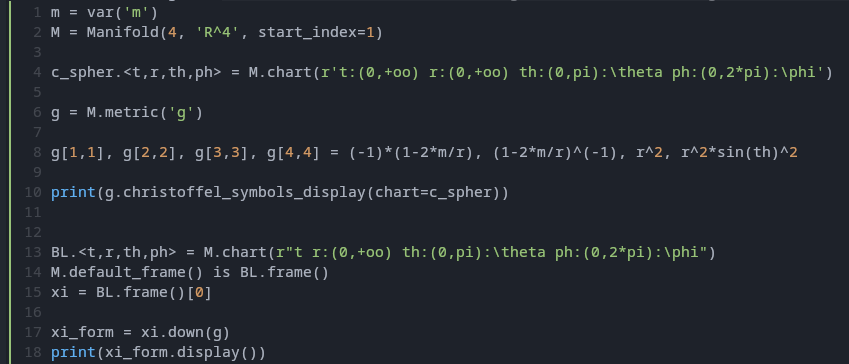
\includegraphics[width=0.95\textwidth]{sage.png}
  \end{center}
\end{figure}
\end{frame}


%%%%%%%%%%%%%%%%%%%%%%%%%%%%%%%%%%%%%%%%%%


\begin{frame}
\frametitle{Geodésicas de Schwarzschild}
Símbolo de Christoffel para la métrica: 
\begin{gather*}
\begin{array}{lcl} \Gamma_{ \phantom{\, t} \, t \, r }^{ \, t \phantom{\, t} \phantom{\, r} } & = & -\frac{M}{2 \, M r - r^{2}} \\ \Gamma_{ \phantom{\, r} \, t \, t }^{ \, r \phantom{\, t} \phantom{\, t} } & = & -\frac{2 \, M^{2} - M r}{r^{3}} \\ \Gamma_{ \phantom{\, r} \, r \, r }^{ \, r \phantom{\, r} \phantom{\, r} } & = & \frac{M}{2 \, M r - r^{2}} \\ \Gamma_{ \phantom{\, r} \, {\theta} \, {\theta} }^{ \, r \phantom{\, {\theta}} \phantom{\, {\theta}} } & = & 2 \, M - r \\ \Gamma_{ \phantom{\, r} \, {\phi} \, {\phi} }^{ \, r \phantom{\, {\phi}} \phantom{\, {\phi}} } & = & {\left(2 \, M - r\right)} \sin\left({\theta}\right)^{2} \\ \Gamma_{ \phantom{\, {\theta}} \, r \, {\theta} }^{ \, {\theta} \phantom{\, r} \phantom{\, {\theta}} } & = & \frac{1}{r} \\ \Gamma_{ \phantom{\, {\theta}} \, {\phi} \, {\phi} }^{ \, {\theta} \phantom{\, {\phi}} \phantom{\, {\phi}} } & = & -\cos\left({\theta}\right) \sin\left({\theta}\right) \\ \Gamma_{ \phantom{\, {\phi}} \, r \, {\phi} }^{ \, {\phi} \phantom{\, r} \phantom{\, {\phi}} } & = & \frac{1}{r} \\ \Gamma_{ \phantom{\, {\phi}} \, {\theta} \, {\phi} }^{ \, {\phi} \phantom{\, {\theta}} \phantom{\, {\phi}} } & = & \frac{\cos\left({\theta}\right)}{\sin\left({\theta}\right)} \end{array}
\end{gather*}
\end{frame}


%%%%%%%%%%%%%%%%%%%%%%%%%%%%%%%%%%%%%%%%%%


\begin{frame}
\frametitle{Geodésicas de Schwarzschild}

Reemplazando los símbolos de Christoffel en la ecuación de la geodésica: 
\begin{gather*}
  \ddot t + \frac{2M}{r(r-2M)}\dot r \dot t = 0\\
  \ddot r + \frac{M}{r^3}(r-2M)\dot t^2 - \frac{M\dot r}{r(r-2M)}-(r-2M)\dot \phi^2=0 \\
  \ddot \phi + \frac{2}{r} \dot \phi \dot r = 0 
\end{gather*}
\end{frame}


%%%%%%%%%%%%%%%%%%%%%%%%%%%%%%%%%%%%%%%%%%


\begin{frame}
\frametitle{Intervalo Luminoide}
Como estamos en un intervalo luminoide podemos hacer $ ds^2 = 0  $ por lo que la métrica nos queda: 
\begin{gather*}
  - \left(1 - \frac{2GM }{r }\right)dt^2 + \left(1 - \frac{2GM }{r}\right) ^ {-1 } dr^2 + r^2 d \Omega^2 = 0 
\end{gather*}
Haciendo el reemplazo $ u = \frac{1}{r} $ nos queda: 
\begin{gather*}
  \left(\frac{d u  }{d \phi }\right)^2 = 2M u^3 - u^2 + \frac{1}{b^2 } 
\end{gather*}
A $ b  $ se le conoce como parámetro de impacto y nos determina la forma de la orbita. $ b = \sqrt{27 } M  \rightarrow $ orbitas de circunferencia inestable. $ b < \sqrt{27 } M  $ orbitas de caída en el centro.
\end{frame}


%%%%%%%%%%%%%%%%%%%%%%%%%%%%%%%%%%%%%%%%%%


\begin{frame}
  \section{Referencias}
  \nocite{*}

  \bibliographystyle{ieeetr}
  \bibliography{ref}
\end{frame}
\end{document}
